\selectlanguage{greek}
\chapter*{Εκτεταμένη Περίληψη}
\addcontentsline{toc}{chapter}{Εκτεταμένη Περίληψη}
\section*{Κίνητρο}

Σήμερα, συναντάμε την εικονοποίηση υπολογιστών στα περισσότερα από τα υπολογιστικά περιβάλλοντα. Αυτό προέρχεται από το γεγονός ότι μπορεί κανείς να απομονώσει τελείως το τρέχον περιβάλλον, συνεπώς το μηχάνημα του \en host\gr{} μένει ανέπαφο, πράγμα το οποίο είναι εξαιρετικά ωφέλιμο για την ανάπτυξη λογισμικού. Επιπλέον, στον κόσμο της ανάπτυξης ιστότοπων, η εικονοποίηση είναι κάτι απολύτως απαραίτητο, το οποίο παρακινεί τις εταιρίες να βελτιστοποιήσουν το κόστος των λειτουργιών των \en servers\gr{}.

Το \en Docker\gr{} έφερε την επανάσταση στην εικονοποίηση, καθώς καθιστά εφικτό το \say{πακετάρισμα} μιας εφαρμογής, με όλες τις εξαρτήσεις της, σε ένα ελαφρύ \en container\gr{}. Η εικονοποίηση που υλοποιεί το \en Docker\gr{} ονομάζεται εικονοποίηση επιπέδου λειτουργικού συστήματος ή εικονοποίηση βασισμένη σε \en container\gr{}, αφού τα μηχανήματα των \en guest\gr{} που υλοποιούνται ονομάζονται επίσης \en containers\gr{}. Ανεξάρτητα από την πρόσφατη, αναπάντεχη επιτυχία και την εκρηκτική εξάπλωση του \en Docker\gr{}, τα \en containers\gr{} είναι ένα χαρακτηριστικό που προϋπήρχε, αλλά η χρήση τους για εύκολη ανάπτυξη και αξιοποίηση εφαρμογών ήταν μια νέα πτυχή τους που εισήγαγε το \en Docker\gr. Στις μέρες μας, το \en Docker\gr{} είναι η πιο δημοφιλής πλατφόρμα για \en containers\gr{}, καθώς βελτιώνει την εικονοποίση αυτού του τύπου, εισάγοντας κάποιες χρήσιμες νέες έννοιες, όπως περιγραφικά αρχεία ρυθμίσεων και την δυνατότητα να επικυρώσεις τις ενημερώσεις κάποιου πάνω σε ένα \en container\gr.

Το \en Docker\gr{} έγινε περίφημο, κυρίως λόγω της ταχύτητας και της μεταφερσιμότητας του. Σε αντίθεση με την εικονοποίηση υλικού (όπως \en VMware ESXi\gr{} ή \en QEMU\gr{}), η εικονοποίηση λειτουργικού επιπέδου έρχεται με ελαφρύτερο φορτίο, συγκριτικά με την εικονοποίηση υλικού. Επειδή τα \en containers\gr{} δεν απαιτούν την εκκίνηση του λειτουργικού συστήματος, ξεκινούν σε λιγότερο από ένα δευτερόλεπτο και η απόδοσή τους είναι πολύ κοντά στην απόδοση με τους επόπτες τύπου 1. Σχετικά με τη μεταφερσιμότητα, ένα \en container\gr{} \say{πακετάρει} μια εφαρμογή μαζί με ό,τι αυτή χρειάζεται για να τρέξει, όπως τα αρχεία ρυθμίσεων και εξαρτήσεις. Αυτό καθιστά δυνατή μια εύκολη και αξιόπιστη εκτέλεση εφαρμογών σε διαφορετικά περιβάλλοντα και, χωρίς να έχει σημασία πόσο περίπλοκη μπορεί να είναι η κάθε εφαρμογή, μπορεί να \say{πακεταριστεί} σαν \en container\gr.
 
Υπο το φως των παραπάνω, είναι ξεκάθαρο ότι αυτά τα πλεονεκτήματα αποτελούν τους βασικούς λόγους για τους οποίους εταιρίες, συμπεριλαμβανομένων μεγάλων ονομάτων όπως \en Paypal, Visa, Ebay, Netflix, Yelp, Spotify\gr{} κ.ά, υιοθετούν το \en Docker\gr{} με αξιοσημείωτους ρυθμούς.

Κοιτώντας την άλλη πλευρά του νομίσματος βέβαια, αν τα \en docker containers\gr{} δεν χρησιμοποιούνται με σύνεση και με ασφάλεια, είναι πολύ πιο εύκολο να κάνουν την εμφάνιση τους απειλές και ευπάθειες, απ'ότι είναι στα εικονικά μηχανήματα. Είναι ασφαλές να πούμε ότι τα εικονικά μηχανήματα είναι πιο ασφαλή, αφού τα \en containers\gr{} χρησιμοποιούν κλήσεις συστήματος κατευθείαν προς τον πυρήνα. Αυτό οδηγεί σε μια εκτεταμένη ομάδα αδυναμιών και ευπαθειών, ειδικά σε σχέση με το θέμα της απομόνωσης \en(isolation)\gr. 

Παρά τα πλεονεκτήματα του \en Docker\gr{}, η απομόνωση των \en containers (isolation)\gr{} είναι ένας συμβιβασμός που πρέπει να γίνει. Ενώ είναι απολύτως εφικτό να απομονώσει κανείς τα \en Docker containers\gr{} όπως τα εικονικά μηχανήματα, τα περισσότερα καθιερωμένα \en Docker containers\gr{}, εκείνα δηλαδή που τρέχουν σε μια βασική κοινότητα ή σε μια εμπορική μηχανή του \en Docker\gr{} στα \en Linux\gr{}, δεν είναι απομονωμένα το ένα από το άλλο, όπως είναι τα εικονικά μηχανήματα.

Στην παρούσα διπλωματική, απευθυνόμαστε στην ανησυχία που πηγάζει σχετικά με την απομόνωση του \en Docker\gr{}, προστατεύοντας τα \en Docker containers\gr{}, μέσω της χρήσης Συστήματος Υποχρεωτικού Ελέγχου \en (MAC)\gr. Το σύστημα \en MAC\gr{} στο οποίο εστιάζουμε είναι το \en AppArmor\gr{}. Το \en AppArmor\gr{} είναι ένα \en Linux security module (LSM)\gr{}, που σημαίνει ότι είναι μια ενίσχυση πυρήνα, η οποία προστατεύει το λειτουργικό σύστημα και τις εφαρμογές του από απειλές στην ασφάλεια, περιορίζοντας τα προγράμματα σε μια οριοθετημένη ομάδα από πόρους με χρήση των λεγόμενων \en profiles\gr{}. Εμείς αναπτύξαμε ένα λογισμικό το οποίο δημιουργεί \en profiles\gr{} για τα \en docker services\gr{}, τα οποία είναι προσαρμοσμένα στο έργο κάθε εφαρμογής, υπό τον κανόνα των ελάχιστων προνομιών, προκειμένου να διατηρίσουμε την απομόνωση, περιορίζοντας τις επιτρεπόμενες πράξεις ενός \en container.\gr{}

\section*{Συνεισφορά}
Οι κύριες συνεισφορές αυτής της εργασίας είναι οι ακόλουθες:
\begin{enumerate}
\item Σχεδίαση και υλοποίηση ενός λογισμικού ανοικτού κώδικα, με το όνομα \en SecureWilly\gr{}\footnote{Ο πηγαίος κώδικας είναι διαθέσιμος στο \en Github repository \url{https://github.com/FaniD/SecureWilly}}\gr{}, το οποίο δημιουργεί \en profile\gr{} για μία εφαρμογή, είτε αυτή έχει ένα \en service\gr{} είτε περισσότερα, προκειμένου να προστατεύσει τα \en containers\gr{} και να διατηρίσει την απομόνωση τους.
\item Ενώ υπάρχουν κι άλλα προγράμματα που δημιουργούν \en profiles\gr{}, το \en SecureWilly\gr{} είναι το πρώτο πρόγραμμα που χειρίζεται εφαρμογές με πολλαπλά \en services\gr{} και παράγει ένα \en profile\gr{} για κάθε \en service\gr{}, λαμβάνοντας υπόψην την συνεργασίας μεταξύ τους.
\item Εξονυχιστική έρευνα για τα ευπαθή χαρακτηριστικά του \en docker\gr{}, τα οποία μπορεί να οδηγήσουν σε επιθέσεις και λεπτομερής ανάλυση καθενός από αυτά.
\item Αρκετά παραδείγματα από επιθέσεις \en container breakout\gr{} έχουν υλοποιηθεί, στα πλαίσια ηθικού \en hacking\gr{}, προκειμένου να ενισχύσουμε την ασφάλεια.
\item Προειδοποιήσεις στον χρήστη σχετικά με ευπάθειες που βρέθηκαν στο \en docker project\gr{} και οι οποίες θα μπορούσαν να οδηγήσουν σε κάποια επίθεση, όπως η χρήση του \en privileged mode \gr{} ή η είσοδος στα \en namespaces\gr{} του \en host \gr{}.
\item Δημιουργία \en AppArmor profiles\gr{} για μια περίπτωση της πλατφόρμας \en Nextcloud\gr{} (δύο \en profiles\gr{} δημιουργήθηκαν, ένα για την εφαρμογή του \en nextcloud\gr{} και ένα για την βάση δεδομένων που χρησιμοποιεί), σαν παράδειγμα στην πειραματική αξιολόγηση.
\end{enumerate}

\section*{Περιγραφή κεφαλαίων}
Στην επόμενη ενότητα του \textbf{Κεφαλαίου 1}, περιγράφουμε εν συντομία τα βασικά χαρακτηριστικά του \en SecureWilly\gr{}, του λογισμικού που δημιουργήσαμε, και τις φάσεις της ανάπτυξής του.

Το \textbf{Κεφάλαιο 2} εστιάζει στην εικονοποίηση με \en containers\gr{}, το \en Docker\gr{} και τα εργαλεία ασφάλειας που υπάρχουν προκειμένου να το προστατεύσουν. 

Το \textbf{Κεφάλαιο 3} περιγράφει την ανάπτυξη του \en SecureWilly\gr{}, προκειμένου να παράγουμε με αυτόματο τρόπο ασφαλή και αποδοτικά \en AppArmor profiles\gr{}, για κάθε service ενός \en docker project\gr. 

Το \textbf{Κεφάλαιο 4} μελετά τις επιθέσεις που μπορούν να διαπραχθούν στα \en containers\gr{}, ειδικά όταν σχετίζονται με την παραβίαση της απομόνωσης μεταξύ του \en host\gr{} και των \en containers\gr{}. Αρκετές τεχνικές οι οποίες μπορούν να χρησιμοποιηθούν για να διαπραχθούν αυτές οι επιθέσεις περιγράφονται και εξηγείται πώς μπορεί να χρησιμοποιηθεί το \en SecureWilly\gr{} προκειμένου να τις αποτρέψει, είτε μέσω της προσθήκης κανόνων στα \en AppArmor profiles\gr{} είτε μέσω της διάθεσης προειδοποιήσεων προς το χρήστη.

Το \textbf{Κεφάλαιο 5} δείχνει τα αποτελέσματα της χρήσης του \en SecureWilly\gr{} στα \en benchmarks\gr{} του \en CloudSuite\gr{} και στο \en Nextcloud\gr{} και αξιολογείται η λειτουργικότητα, η απόδοση και η επεκτασιμότητα του \en SecureWilly\gr{}. Τα \en profiles\gr{} που παράγονται από το \en SecureWilly\gr{} συγκρίνονται με το αντίστοιχο \en profile\gr{} που δημιουργήθηκε μέσω του εργαλείου \en genprof\gr{}. Ο χρόνος που προστίθεται από τη χρήση του \en AppArmor\gr{} υπολογίστηκε, μετρώντας τον χρόνο για ένα από τα παραδείγματα που υλοποιήσαμε.

Το \textbf{Κεφάλαιο 6} συνοψίζει τα βασικά συμπεράσματα αυτής της εργασίας, δείχνει σχετικά λογισμικά που υπάρχουν και δίνει συμβουλές για μελλοντική ανάπτυξη του \en SecureWilly\gr{}.

\section*{Σύντομη περιγραφή του λογισμικού}
Το \en SecureWilly\gr{} είναι το λογισμικό που δημιουργήσαμε προκειμένου να παράγουμε με αυτόματο τρόπο \en profile\gr{} για \en docker projects\gr{}.

Χειρίζεται τόσο \en projects\gr{} με ένα \en service\gr{}, όσο και με πολλαπλά και σέβεται την συνεργασία μεταξύ τους, πράγμα το οποίο αντικατοπτρίζεται στους κανόνες των \en AppArmor profiles\gr{}.

Τα \en profiles\gr{} δημιουργούνται για κάθε \en container\gr{} και ακολουθούν την αρχή των ελάχιστων προνομιών. Αυτή η αρχή απαιτεί σε ένα αφηρημένο στρώμα υπολογιστικού περιβάλλοντος ότι κάθε οντότητα - διεργασία, χρήστης ή πρόγραμμα - πρέπει να μπορεί να έχει πρόσβαση μόνο στις πληροφορίες και τους πόρους που του είναι απαραίτητοι για τον σκοπό του. Αυτό επιβεβαιώνει ότι κάθε \en profile\gr{} περιορίζει στο μεγαλύτερο δυνατό βαθμό τα εκάστοτε \en services\gr{} και επιτρέπει αποκλειστικά τις απαραίτητες λειτουργίες του έργου του, ενώ απαγορεύει κάθε περιττή ενέργεια. Συνεπώς, τα \en profiles\gr{} που παράγονται είναι ασφαλή και προστατεύουν την απομόνωση του \en host\gr{} και των \en containers\gr{}.

Εκτός από τον πρωταρχικό στόχο του \en SecureWilly\gr{} που είναι η δημιουργία των \en AppArmor profiles\gr{}, παράγονται επίσης διάφορα άλλα χρήσιμα στοιχεία σχετικά με το \en docker project \gr{} που δίνεται ως είσοδος, όπως προειδοποιήσεις σχετικά με ευπάθειες που εντοπίζονται, αρχεία \en yml\gr{} για κάθε \en service\gr{} στην περίπτωση που δεν υπάρχει ήδη \en docker-compose\gr{} αρχείο καθώς και γραφήματα που αναπαριστούν την συμπεριφορά του κάθε \en service\gr{} μέσα από τους κανόνες των \en profiles\gr{} που παράχθηκαν.

Η ανάπτυξη του \en SecureWilly\gr{} χωρίζεται σε δύο φάσεις:
\begin{itemize}
\item Στην πρώτη φάση, δύο αναλυτές χρησιμοποιούνται σε δύο διαφορετικού τύπου αναλύσεις, προκειμένου να εξάγουν κανόνες για τα \en profiles\gr{}. Η στατική ανάλυση και ο αναλυτής της χειρίζεται τον αρχικό κώδικα του \en docker project\gr{}, ο οποίος δίνεται από τον χρήστη, και παράγει ένα προκαταρκτικό \en profile\gr{}, το οποίο περιέχει μια ελάχιστη ομάδα από εξαγόμενους κανόνες από τον κώδικα. Στη συνέχεια, η δυναμική ανάλυση παίρνει μέρος και ο αναλυτής της δέχεται το προκαταρκτικό \en profile\gr{} της στατικής ανάλυσης και το χρησιμοποιεί για να εξασκήσει το \en docker project\gr{} και να εξάγει νέους κανόνες, παρακολουθώντας τα \en logs\gr{} του συστήματος.

\item Στη δεύτερη φάση, χρησιμοποιούμε την τεχνική του \en reverse engineering\gr{} κάνοντας επιθέσεις τύπου \en container breakout\gr{}, στα πλαίσια ηθικού \en hacking\gr{}, προκειμένου να δημιουργήσουμε κανόνες που αποτρέπουν αυτές τις επιθέσεις και προστατεύουν τα \en docker containers\gr{}. Αυτό οδηγεί στο να προσθέτουμε μερικούς σταθερούς κανόνες στο προκαταρκτικό \en profile \gr{} καθώς και στο να παράγουμε προειδοποιήσεις σχετικά με τις ευπάθειες που εντοπίζονται.
\end{itemize}

\section*{Σχεδίαση και υλοποίηση του λογισμικού}

Το λογισμικό που δημιουργήσαμε έχει σαν πρωταρχικό στόχο την αυτόματη δημιουργία \en AppArmor profiles\gr{} για το \en docker project\gr{} που δέχεται σαν είσοδο. Τα \en profiles\gr{} που δημιουργούνται είναι πλήρως προσαρμοσμένα στο \en docker project\gr{}, με βάση την αρχή των ελάχιστων προνομιών, δηλαδή επιτρέπουν αποκλειστικά μια ομάδα από ενέργειες, οι οποίες προσδιορίζονται μέσα από ένα πλάνο χρήσης που δίνεται από τον χρήστη. Κάθε άλλη ενέργεια θα θεωρηθεί περιττή και θα αποκλειστεί. Το λογισμικό μας επίσης υποστηρίζει \en docker projects\gr{} με πολλαπλά \en services\gr{} και παράγει ένα \en AppArmor profile\gr{} για κάθε ένα από αυτά. Τα \en profiles\gr{} που παράγονται για κάθε \en service\gr{} περιέχουν κανόνες που αναφέρονται στην συνεργασία μεταξύ τους, με τον τρόπο που αυτή υποδεικνύεται από το πλάνο χρήσης. Το \en SecureWilly\gr{} εστιάζει στη διατήρηση της απομόνωσης μεταξύ του \en host\gr{} και των \en containers\gr{} καθώς και μεταξύ των \en containers\gr{}.

Όπως αναφέραμε και προηγουμένως, εκτός από τα \en AppArmor profiles\gr{}, παράγονται κάποια επιπλέον στοιχεία σχετικά με το \en docker project\gr{}: προειδοποιήσεις για τις ευπάθειες που εντοπίζονται, αρχεία \en yml\gr{} για κάθε \en service\gr{} και γραφήματα/μετρικές σχετικά το ρόλο του κάθε \en service\gr{} όπως φαίνεται μέσα τους κανόνες του αντίστοιχου \en profile\gr{}.

Η παρακάτω εικόνα αναπαριστά την αρχιτεκτονική του \en SecureWilly. 
\begin{figure}[h!]
   \centering
   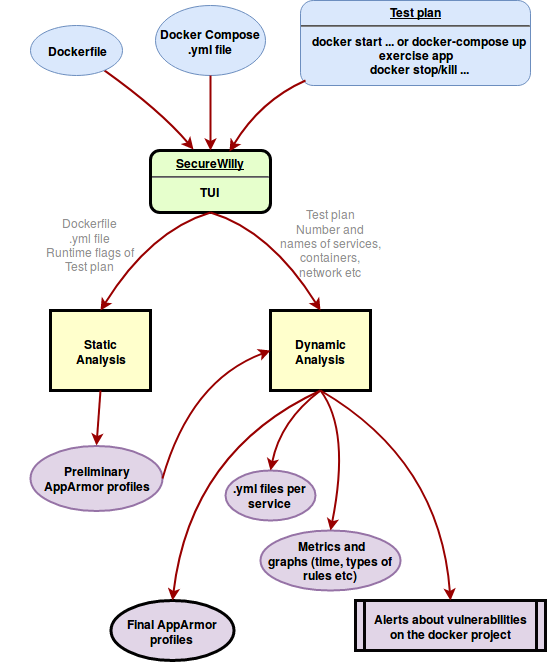
\includegraphics[width=0.6\linewidth]{figures/SecureWilly.png}
 %%  \caption{SecureWilly}
\end{figure}
\gr
\subsection*{Διεπαφή χρήστη}
Η διεπαφή χρήστη του λογισμικού μας, είναι σχετικά απλή και αναπαρίσταται μέσω τερματικού.

Το \en SecureWilly\gr{} απαιτεί σαν είσοδο κάποιες πληροφορίες σχετικά με το \en docker project\gr{} από τον χρήστη ενώ τον καθοδηγεί μέσω μηνυμάτων σχετικά με το πώς πρέπει να δώσει την κάθε πληροφορία. Οι πληροφορίες που ζητά είναι οι εξής:
\begin{itemize}
\item Αριθμό των \en services\gr{}.
\item Ονόματα των \en services\gr{}.
\item Το \en path\gr{} του \en Dockerfile\gr{} από κάθε \en service/image\gr{} αν υπάρχει, αλλιώς ο χρήστης πρέπει να γράψει \say{Ν}.
\item Το \en path\gr{} του \en docker-compose file (.yml file)\gr{} αν υπάρχει, αλλιώς ο χρήστης πρέπει να γράψει \say{Ν}.
\item Το όνομα του εσωτερικού \en network\gr{} αν χρειάζεται το \en docker project\gr{}, αλλιώς ο χρήστης πρέπει να γράψει \say{Ν}.
\item Εντολές για ένα πλάνο χρήσης, αντιπροσωπευτικό του τι χρειάζεται να κάνει η εφαρμογή, που να περιλαμβάνει και τις εντολές εκκίνησης των \en docker containers\gr{} καθώς και τις εντολές τερματισμού τους.
\end{itemize}

Στη συνέχεια, επεξεργάζεται τα δεδομένα που έλαβε ως είσοδο, έτσι ώστε να ετοιμάσει τα δεδομένα που χρειάζονται οι αναλυτές που χρησιμοποιεί στη συνέχεια.

Η έξοδος που παράγει μετά την εκτέλεση των δύο αναλύσεων αποτελείται από τα εξής:
\begin{itemize}
\item Ένα \en AppArmor profile\gr{} για κάθε \en service\gr{} του \en docker project\gr{}.
\item Ένα \en yml file\gr{} για κάθε \en service\gr{} του \en docker project\gr{}.
\item Γραφήματα σχετικά με τον ρόλο του κάθε \en service\gr{} του \en docker project\gr{} ανάλογα με τους κανόνες που εμφανίζονται στο αντίστοιχο \en profile\gr{}.
\item Αρχεία προειδοποιήσεων για εμφάνιση ευπαθειών στο \en docker project\gr{}. Αυτή τη στιγμή, έχουν υλοποιηθεί τα αρχεία για \en containers\gr{} που τρέχουν σε \en privileged mode\gr{} και που εισέρχονται στο \en namespace\gr{} του \en host\gr{}. 
\end{itemize}

\subsection*{Στατική Ανάλυση}
Στη φάση της στατικής ανάλυσης, το λογισμικό που δημιουργήσαμε αναλύει τον κώδικα μέσω του οποίου δημιουργείται το \en docker image\gr{} και ρυθμίζονται τα \en docker containers\gr{}, έτσι ώστε να παραχθούν κάποιοι πρώτοι κανόνες και να δημιουργήσουμε ένα προκαταρκτικό \en profile\gr. Πιο συγκεκριμένα, ο κώδικας που αναλύεται είναι:\en
\begin{enumerate}
\item Dockerfile
\item Docker compose file (.yml)
\item Flags\gr{} που χρησιμοποιούνται κατά τη διάρκεια του χρόνου εκτέλεσης
\end{enumerate}
\gr{}
Τα παραπάνω αρχεία, υφίστανται μια επεξεργασία κειμένου και μέσα από τις εντολές τους σχηματίζονται οι αντίστοιχοι κανόνες που αποτελούν το πρώτο \en profile\gr{} για κάθε \en service\gr{} του \en docker project\gr{}.

\subsection*{Δυναμική Ανάλυση}
Στη φάση της δυναμικής ανάλυσης, το \en SecureWilly\gr{} χρησιμοποιεί μια έκδοση του \en AppArmor profile\gr{} που σταδιακά δημιουργεί και παρακολουθεί τα \en logs\gr{} του συστήματος, ώστε μέσα από αυτά να σχηματίσει νέους κανόνες. 

Στον πρώτο γύρο θα χρησιμοποιήσει το \en profile\gr{} που δημιουργήθηκε από την στατική ανάλυση και στη συνέχεια θα προσθέσει τους κανόνες που εξάγονται από τα \en logs\gr{} του συστήματος. Η διαδικασία αυτή θα επαναλαμβάνεται, χρησιμοποιώντας κάθε φορά το \en profile\gr{} που δημιουργήθηκε στον προηγούμενο γύρο μέχρι να μην μπορούν να εξαχθούν νέοι κανόνες από τα \en logs\gr. 

Μέσα στην παραπάνω επαναληπτική διαδικασία, το \en SecureWilly\gr{} τρέχει το πλάνο χρήσης που δόθηκε από το χρήστη. Το \en AppArmor profile\gr{} είναι σε \en complain mode\gr{}. Όταν δεν είναι δυνατό να εξαχθούν νέοι κανόνες από τα \en logs\gr{} τότε το \en profile\gr{} θα τεθεί σε \en enforce mode\gr{}, θα εκτελεστεί ξανά το πλάνο χρήσης και αν βρεθούν νέοι εξαγόμενοι από τα \en logs\gr{} κανόνες, τότε η διαδικασία θα επαναληφθεί από την αρχή με το \en profile\gr{} και πάλι σε \en complain mode\gr{}, αν όχι, τότε η δυναμική ανάλυση έχει τελειώσει και έχουμε το τελικό \en profile\gr{} για κάθε \en service\gr{}.

\subsection*{Στόχος πρώτης φάσης}
Τελικά το \en SecureWilly\gr{} καταφέρνει να δημιουργήσει \en AppArmor profiles\gr{} πλήρως προσαρμοσμένα στο δοσμένο \en docker project\gr{}, αφότου λάβει τις απαραίτητες πληροφορίες περί αυτού από τον χρήστη. Η στατική ανάλυση είναι υπεύθυνη για τη δημιουργία κανόνων οι οποίοι καθιστούν το \en profile\gr{} ασφαλές καθώς προσθέτει αυστηρούς κανόνες σχετικά με τη ρύθμιση των \en containers\gr{}, ενώ η δυναμική ανάλυση εμπλουτίζει αυτό \en profile\gr{} με κανόνες οι οποίοι αντιπροσωπεύουν τις απαιτήσεις του \en project\gr{} και κάνουν το \en profile\gr{} της στατικής ανάλυσης πιο αυστηρό και πιο αποδοτικό.

Η πρώτη φάση της ανάπτυξης του λογισμικού εστιάζει κυρίως στο ίδιο το \en project\gr. Ανεξάρτητα όμως από την αποδοτικότητα του \en profile\gr{} που δημιουργήθηκε σε αυτή τη φάση, η απομόνωση μπορεί ακόμα να καταπατηθεί. Αυτό μας οδήγησε στη δεύτερη φάση ανάπτυξης του λογισμικού, η οποία εστιάζει στην αντιμετώπιση επιθέσεων σχετικών με την απομόνωση που μπορούν να διαπραχθούν από και προς τα \en containers\gr{} και πώς μπορεί το \en SecureWilly\gr{} να τις αποτρέψει. Η επόμενη ενότητα αφορά τη δεύτερη φάση του λογισμικού, η οποία ολοκληρώνει την ανάπτυξη του.

\section*{Επιθέσεις και ευπάθειες}
Ανάμεσα στους στόχους του λογισμικού που δημιουργήσαμε, είναι και η επίτευξη της απομόνωσης μεταξύ του \en host\gr{} και του \en container\gr{}. Η διατήρηση της απομόνωσης είναι μία σημαντική πτυχή της διατήρησης της συνολικής ασφάλειας στο \en docker\gr{}, καθώς διάφορες επιθέσεις μπορούν να επιτευχθούν, αν η απομόνωση παραβιαστεί.

Μια εξονυχιστική έρευνα έγινε πάνω στις επιθέσεις οι οποίες μπορεί να συμβούν, αν τα \en docker containers\gr{} δεν είναι αρκετά ασφαλή. Επισημάναμε μια ομάδα ευπαθειών οι οποίες μπορεί να οδηγήσουν σε επιθέσεις και στα πλαίσια του ηθικού \en hacking\gr{}, υλοποιήσαμε συγκεκριμένα παραδείγματα επιθέσεων, τα οποία δοκιμάστηκαν σε πραγματικά συστήματα.

Μέσω της τεχνικής του \en reverse engineering\gr{}, καταφέραμε να δημιουργήσουμε κανόνες τους οποίους το \en SecureWilly\gr{} προσθέτει στα \en AppArmor profiles\gr{} που δημιουργεί, προκειμένου να βοηθήσει την απομόνωση. Αυτή τη στιγμή, το \en SecureWilly\gr{} αποτρέπει επιτυχώς τις επιθέσεις που γίνονται με το εργαλείο \en nsenter\gr{} καθώς και αυτές του \en Docker group\gr{}. Για τις υπόλοιπες ευπάθειες τις οποίες δεν μπορούν τα παραχθέντα \en profiles\gr{} να αντιμετωπίσουν, το \en SecureWilly\gr{} παράγει προειδοποιήσεις για ό,τι ευπάθειες εντοπιστούν στα \en docker containers\gr{}, έτσι ώστε ο χρήστης να τις αποφύγει και να χρησιμοποιήσει καλύτερες πρακτικές.

Ο τύπος των επιθέσεων στον οποίο εστιάσαμε, ονομάζεται \en container breakout\gr{} και αφορά \en containers\gr{} τα οποία σπάνε τα \en namespaces\gr{} τους και προσπαθούν να εισβάλλουν στον χώρο του \en host\gr{} ή άλλων \en containers\gr{}, πράγμα το οποίο έχει άμεση σχέση με την απομόνωση.

Οι ευπάθειες που εντοπίσαμε στο \en docker\gr{} και οι οποίες μπορούν να οδηγήσουν σε τέτοιου τύπου επιθέσεις είναι οι παρακάτω:
\begin{description}[style=nextline]
\item[Χρήση του \en root\gr{} μέσα σε \en containers]
Ο χρήστης \en root\gr{} έχει πρόσβαση σε όλο το \en filesystem\gr{} του \en container\gr{}, ενώ συνήθως έχει και πιο πολλές δυνατότητες - \en capabilities\gr{} όπως θα δούμε παρακάτω - από έναν απλό χρήστη και συνεπώς είναι πιο εύκολο να κάνει μια επίθεση, απ'ότι κάποιος άλλος χρήστης. Στις περισσότερες περιπτώσεις μάλιστα, ο χρήστης \en root\gr{} δεν έχει λόγο να χρησιμοποιείται, άρα αποτελεί μια ευπάθεια χωρίς λόγο.

Για να απαντήσουμε στο ερώτημα αν ο χρήστης \en root\gr{} του \en host\gr{} είναι ο ίδιος με τον \en root\gr{} του \en container\gr{}, υλοποιήσαμε μερικά απλά παραδείγματα, χωρίς να ενεργοποιήσουμε το \en user namespace\gr{} στο \en docker\gr{}. Η απάντηση είναι πως ναι, ο χρήστης \en root\gr{} είναι ο ίδιος, αν δεν έχουμε ενεργοποιήσει \en user namespace\gr{}.

Ένας κακόβουλος χρήστης που τρέχει σαν \en root\gr{} σε ένα \en container\gr{} μπορεί να χρησιμοποιήσει την ιδιότητα του \en root\gr{} για να εκτελεί \en privileged\gr{} ενέργειες, προκειμένου να επιτεθεί στο μηχάνημα του \en host\gr{}.

Για την αντιμετώπιση της συγκεκριμένης ευπάθειας τα \en user namespaces\gr{} θα μπορούσαν να αποτελέσουν τη λύση. Τα \en user namespaces\gr{}, όπως αναφέρεται στην αντίστοιχη \en man page\gr{}, απομονώνουν αναγνωριστικά και χαρακτηριστικά που σχετίζονται με την ασφάλεια, πιο συγκεκριμένα \en IDs\gr{} των χρηστών και \en IDs\gr{} από \en groups\gr{}, το \en directory\gr{} του \en root\gr{}, κλειδιά και \en capabilities\gr{}. Στο \en Docker\gr{} ωστόσο το \en user namespace\gr{} δεν είναι ενεργοποιημένο από μόνο του, αλλά απαιτεί χειροκίνητη ρύθμιση. Αφού λοιπόν ενεργοποιηθούν, θα παρέχουν προστασία στον χρήστη \en root\gr{} του \en host\gr{} μηχανήματος και είναι σίγουρα ένα ιδιαίτερα χρήσιμο εργαλείο για να χρησιμοποιούμε. Παρ'όλα αυτά, καθώς η εφαρμογή τους αποτελεί μια νέα προσθήκη στο \en docker\gr{}, υπάρχουν κάποια προβλήματα, όπως η εκκαθάριση των \en images\gr{} όταν η εντολή \en userns-remap\gr{} χρησιμοποιείται. Ένας άλλος λόγος που τα \en user namespaces\gr{} ίσως αποτύχουν να παρέχουν προστασία είναι η περίπτωση κάποιο μέρος του κώδικα του πυρήνα να μην είναι προσαρμοσμένα στο να λειτουργεί για διαφορετικά \en user namespaces\gr{} και έτσι να προκληθεί βλάβη στο περιβάλλον του \en host\gr{}.

Συνεπώς, τα \en user namespaces\gr{} είναι ένα χρήσιμο εργαλείο για να χρησιμοποιήσουμε, αλλά μόνο του δεν είναι αρκετό για να παρέχει προστασία στο μηχάνημα του \en host\gr{} και έτσι η χρήση του \en root\gr{} εντός των \en containers\gr{} παραμένει μια κακή επιλογή. Αν απαιτείται πραγματικά η χρήση του χρήστη \en root\gr{}, τότε η πρώτη επιλογή είναι να προσπαθήσουμε να \say{μεταμφιέσουμε} έναν απλό χρήστη ώστε να φαίνεται σαν \en root\gr{}, είτε με χρήση \en user namespaces\gr{} είτε με την προσθήκη κάποιων \en capabilities\gr{}. Αν και αυτό δεν είναι αρκετό, τότε θα πρέπει να βεβαιωθούμε ότι γίνεται χρήση και άλλων εργαλείων ασφάλειας, σαν επιπλέον τοίχος ασφαλείας, προκειμένου να ασφαλίσουμε το \en container\gr{}.

\item[\en Capabilities\gr{} του πυρήνα]
Οι \say{ειδικές δυνάμεις} του χρήστη \en root\gr{} έχουν διασπαστεί στα λεγόμενα \en capabilities\gr{} πυρήνα. Ένας χρήστης διαθέτει μια υποομάδα από αυτές τις δυνάμεις. Στην περίπτωση του \en docker\gr{} μπορούμε να προσθέσουμε \en capabilities\gr{} στον χρήστη όπως και να αφαιρέσουμε. Τα \en AppArmor profiles\gr{} μπορούν να περιορίσουν ποια \en capabilities\gr{} θα επιτραπούν και ποιά όχι.

Το σύστημα των \en capabilities\gr{} σχεδιάστηκε ώστε να εξαληφθούν τα προβλήματα που σχετίζονται με την ανάγκη των \en privileges\gr{} του χρήστη \en root\gr{}. Μια εφαρμογή μπορεί να ζητάει περισσότερα \en privileges\gr{} αλλά αυτό δεν σημαίνει ότι χρειάζεται να τρέξει αποκλειστικά με χρήστη \en root\gr{}. Μπορούμε απλά να προσθέσουμε το αντίστοιχο \en capability\gr{} που χρειάζεται ο απλός χρήστης. Σε αυτό το σημείο όμως, μπορεί να οδηγηθούμε εύκολα σε σημείο ευπάθειας, καθώς ένας απλός χρήστης μπορεί εύκολα να ανελιχθεί σε χρήστη \en root\gr{} αν προσθέσουμε πολλά \en capabilities\gr{}, και όπως εξηγήσαμε προηγουμένως, η χρήση \en root\gr{} εντός του \en container\gr{} θα ήταν συνετό να αποφεύγεται.

Στις ρυθμίσεις ενός \en docker container\gr{} υπάρχει και η επιλογή του \en privileged mode\gr{}, η οποία ουσιαστικά σημαίνει - μεταξύ άλλων - την προσθήκη όλων των \en capabilities\gr{} στον χρήστη. Προφανώς, αυτή η περίπτωση ταυτίζεται με την περίπτωση της χρήσης του \en root\gr{} και αποτελεί μια ισοδύναμη ευπάθεια, αλλά και μεγαλύτερη αν αναλογιστούμε ότι το \en privileged mode\gr{} παρέχει και άλλες δυνατότητες στα \en containers\gr{}.

Μελετήθηκαν συγκεκριμένα παραδείγματα από \en capabilities\gr{} τα οποία θεωρούνται πιο κρίσιμα ως προς το να οδηγήσουν στην ανέλιξη ενός χρήστη σε \en root\gr{}, όπως το \en SYS\_ADMIN\gr{} κ.ά.

Το \en SecureWilly\gr{} δεν μπορεί να αποτρέψει κάποια επίθεση σχετικά με αυτήν την ευπάθεια, αλλά παρέχει στον χρήστη ειδική προειδοποίηση για τα \en containers\gr{} που χρησιμοποιούν το \en privileged mode\gr{}.

Συνοψίζοντας μπορούμε να επισημάνουμε ότι παρά το γεγονός ότι μια ευρεία χρήση των \en capabilities\gr{} θα μπορούσε να μειώσει τον αριθμό των ευπαθειών, θα πρέπει να προσθέτονται με σύνεση, αλλιώς μπορεί να οδηγήσουν σε επικίνδυνα μονοπάτια.

\item[Απενεργοποίηση των \en namespaces\gr{}]
Τα \en Linux Namespaces\gr{} είναι ένα χαρακτηριστικό το οποίο διαιρεί τους πόρους του πυρήνα και παρέχει απομόνωση μεταξύ τους, όπως για παράδειγμα το \en user namespace\gr{} που είδαμε προηγουμένως. Αυτή τη στιγμή, το \en Linux\gr{} υλοποιεί επτά διαφορετικούς τύπους \en namespaces: mount (mnt), process id (pid), network (net), interprocess communication (ipc), UTS, user id (user), control group (cgroup).\gr{}

Το \en Docker\gr{} χρησιμοποιεί τα \en namespaces \gr{} και τα περισσότερα από αυτά είναι ενεργοποιημένα εξ'αρχής. Μόνο τα \en user namespaces\gr{} είναι απενεργοποιημένα, όπως αναφέραμε και προηγουμένως.

Ένα συχνό φαινόμενο που παρατηρείται κατά τη ρύθμιση των παραμέτρων εκτέλεσης των \en containers\gr{} είναι η είσοδος στα \en namespaces\gr{} του \en host\gr{}. Ο λόγος που αρκετοί χρήστες προβαίνουν σε αυτήν την ενέργεια είναι για να χρησιμοποιήσουν κάποιο μέρος του \en host\gr{} μηχανήματος, όπως το δίκτυο ή το χώρο των διεργασιών, όπως ακριβώς συμβαίνει και με τη χρήση των \en volumes\gr{} για την είσοδο στο \en mount namespace\gr{}. Η ενέργεια αυτή υλοποιείται με την χρήση των αντίστοιχων \en flags\gr{} στις εντολές εκκίνησης των \en docker containers\gr{} ή σαν \en option\gr{} στο \en docker compose file\gr{}.

Από τη στιγμή που ο χρήστης απενεργοποιήσει κάποιο \en namespace\gr{}, ο κίνδυνος για επιθέσεις αυξάνεται αφού όπως είναι προφανές ένας κακόβουλος χρήστης αποκτά άμεση πρόσβαση στο μηχάνημα του \en host\gr{}. Στην περίπτωση αυτή το \en SecureWilly\gr{} δεν μπορεί να κάνει κάτι για να αντιμετωπίσει αυτήν την ευπάθεια, εφόσον δίνεται ρητά από τον χρήστη μέσω του πλάνου χρήσης, παρά μόνο να παρέχει προειδοποιήσεις σχετικά με τα \en containers\gr{} που εισέρχονται στα \en namespaces\gr{} του \en host\gr{}.

Τα \en flags\gr{} που επιτρέπουν την είσοδο στα \en namespaces\gr{} του \en host\gr{} καταστρέφουν κάθε τοίχος απομόνωσης του \en host\gr{} και το κάνουν πιο εύκολο για έναν κακόβουλο χρήστη να εκτελέσει μια επίθεση. Για το λόγο αυτό θα ήταν συνετό να αποφεύγεται η χρήση τους και ο χρήστης να χρησιμοποιεί άλλο τρόπο επικοινωνίας με τον \en host\gr{}. Τα \en namespaces\gr{} υπάρχουν για να μας προστατεύουν γι'αυτό θα ήταν σοφό να σεβόμαστε τα όρια που θέτουν. Αν όλα από αυτά τα \en flags\gr{} χρησιμοποιηθούν, τότε το παιχνίδι έχει ήδη χαθεί. Δεν υπάρχει καν λόγος να χρησιμοποιηθεί το \en docker\gr{} σε αυτήν την περίπτωση, αφού ισοδυναμεί με το να τρέχαμε την εφαρμογή στο \en host\gr{} μηχάνημα. Αν κάποια \en flags\gr{} εξ'αυτών πρέπει να χρησιμοποιηθούν, θα πρέπει να συνδυαστούν με άλλα μέτρα ασφάλειας.

\item[Χρήση του εργαλείου \en nsenter\gr{}]
Το \en nsenter\gr{} είναι το τέλειο εργαλείο για να εκτελέσει ένας κακόβουλος χρήστης μια επίθεση, μπαίνοντας μέσα στα \en namespaces\gr{} μιας άλλης διεργασίας. Το εργαλείο \en nsenter\gr{} διατίθεται μέσω του \en package util-linux\gr{} και ανοίγει τα \en namespaces\gr{} που ζητάει ο χρήστης, δίνοντας πρόσβαση στο \say{εσωτερικό} μιας άλλης διεργασίας. Για τη χρήση του απαιτεί τα \en privileges\gr{} του \en root\gr{} και αυτό αποτελεί έναν ακόμη λόγο για τον οποίο η χρήση του \en root\gr{} θα πρέπει να αποφεύγεται. Το μόνο που χρειάζεται να έχουμε για να το χρησιμοποιήσουμε είναι το \en pid\gr{} της διεργασίας που θέλουμε να εισέλθουμε στα \en namespaces\gr{} της και μετά είμαστε σε θέση να εκτελέσουμε κάθε ενέργεια μέσα σε αυτά. 

Αυτό το εργαλείο μπορεί να χρησιμοποιηθεί για επιθέσεις τύπου \en container breakout\gr{}, ώστε ένα \en container\gr{} να μπορεί να αποκτήσει πρόσβαση στο περιβάλλον τόσο του \en host\gr{} όσο και άλλων \en containers\gr{} που τρέχουν στο ίδιο σύστημα. Αυτό που καθιστά την συγκεκριμένη ευπάθεια ακόμα πιο επικίνδυνη είναι ότι το \en nsenter\gr{} δεν \say{ρίχνει} τα \en capabilities\gr{}. Αυτό σημαίνει ότι το κέλυφος που θα εκκινήσει με τη χρήση του \en nsenter\gr{} μπορεί να επιφέρει δυνητικά μεγαλύτερη βλάβη στον \en host\gr{} από μια απλή διεργασία που τρέχει μέσα στο \en container\gr{}, απλά μέσω της προσθήκης των κατάλληλων \en capabilities\gr{}.

Υλοποιήθηκαν δύο ειδών επιθέσεις:
\begin{itemize}
\item Στην πρώτη ένας κακόβουλος χρήστης επιχειρεί να εισέλθει στο μηχάνημα του \en host\gr{} μέσα από τα \en namespaces\gr{} του \en host\gr{} και να εκτελέσει μια σειρά από εντολές δοκιμάζοντας \en read, write\gr{} και \en execute accesses\gr{}.
\item Στη δεύτερη περίπτωση ένας κακόβουλος χρήστης εκτελεί την ίδια διαδικασία επιχειρώντας να εισέλθει αυτή τη φορά στη διεργασία ενός άλλου \en container\gr{} και στη συνέχεια, όπως και στην πρώτη περίπτωση, δοκιμάζει τα διάφορα \en accesses\gr{} εντός αυτής της διεργασίας.
\end{itemize}

Το \en SecureWilly\gr{} μπορεί να αντιμετωπίσει τις παραπάνω επιθέσεις, καθιστώντας ένα \en container\gr{} μη εντοπίσιμο από άλλα \en containers\gr{}. Αυτό υλοποιείται προσθέτοντας στο \en AppArmor profile\gr{} την εντολή \en deny ptrace(readby, tracedby)\gr{}.

\item[Πρόσβαση στο \en Docker Daemon\gr{}]
Ένα χρήστης ο οποίος έχει πρόσβαση στο \en docker daemon\gr{} έχει τη δυνατότητα να χρησιμοποιήσει το \en docker client\gr{} και να εκτελέσει εντολές στο \en docker\gr{}. Αυτό σημαίνει ότι ο χρήστης αυτός θα μπορούσε να διαχειριστεί τα \en containers\gr{} που τρέχουν στο σύστημα, να εισέλθει στο περιβάλλον τους, να μάθει πληροφορίες για αυτά ή ακόμα και να τα τερματίσει και να δημιουργήσει νέα \en containers\gr{}. Συνεπώς, οι χρήστες που έχουν πρόσβαση στις εντολές του \en docker\gr{} μπορούν να θεωρηθούν αρκετά ισχυροί και για αυτό το λόγο το \en docker CLI\gr{} είναι περιορισμένο να χρησιμοποιείται μόνο από τον \en root\gr{} και τα μέλη του \en docker group\gr{}.

Το \en docker group\gr{} είναι μια ομάδα από χρήστες \en unix\gr{} η οποία δημιουργείται ως μέρος της εγκατάστασης του \en docker\gr{} και είναι το \en owner group\gr{} στα \en file permissions\gr{} της \en unix file socket /var/run/docker.sock.\gr{}

Διάφοροι κίνδυνοι απορρέουν από την προσθήκη χρηστών στο \en docker group\gr{}, οπότε θα πρέπει να είμαστε αρκετά επιλεκτικοί ως προς το ποιός θα γίνει μέλος αυτής της ομάδας.

Σε ένα μηχάνημα που έχει εγκατασταθεί το \en Docker\gr{} οι χρήστες που έχουν πρόσβαση σε αυτό και μπορούν να το χρησιμοποιήσουν είναι όσοι ανήκουν στο \en Docker group\gr{}.

Πιο συγκεκριμένα, ας υποθέσουμε ότι ένα \en container\gr{} τρέχει στο μηχάνημα του \en host\gr{}, χρησιμοποιώντας ένα \en docker image\gr{} ρυθμισμένο ώστε ο χρήστης στην εκκίνηση του \en container\gr{} να είναι ένας απλός χρήστης και όχι \en root\gr{}. Σε μια επίθεση θα μπορούσε κάποιο μέλος του \en docker group\gr{} να εισέλθει στο τρέχον \en container\gr{}, όχι απλά σαν χρήστης αλλά και σαν \en root\gr{} παρά την υπάρχουσα ρύθμιση. Κάτι τέτοιο θα μπορούσε να επιτευχθεί με την εντολή \en docker exec\gr{}. 

Η εντολή αυτή είναι ο τρόπος που παρέχει το \en docker\gr{} για την είσοδο σε ένα τρέχον \en container\gr{}. Το \en docker exec\gr{} ξεκινάει μια διεργασία εντός του \en docker container\gr{} αλλά αυτό που το καθιστά ευπαθές χαρακτηριστικό είναι η δυνατότητα επιλογής οποιουδήποτε χρήστη εντός αυτής της διεργασίας, ακόμα και του \en root\gr{} και όπως εξηγήσαμε παραπάνω, το να τρέχει κάποιος σαν \en root\gr{} εντός του \en container\gr{} μπορεί να αποδειχθεί επικίνδυνο.

Ένα άλλο στοιχείο που μπορεί να ανοίξει το δρόμο για επιθέσεις τύπου \en container breakout\gr{} είναι το να δώσουμε πρόσβαση στα \en containers\gr{} στο \en unix socket /var/run/docker.sock\gr{}. Στο \en Linux\gr{}, τα \en sockets\gr{} χρησιμοποιούνται για να επιτρέπουν σε διαφορετικές διεργασίες να επικοινωνούν μεταξύ τους, έτσι και το \en docker.sock\gr{} χρησιμοποιείται για την επικοινωνία με τη βασική διεργασία του \en docker\gr{}. Αφού όλα στο \en Linux\gr{} θεωρούνται αρχεία, έτσι και τα \en sockets\gr{} είναι αρχεία και επομένως μπορούμε να τα μοιραστούμε μέσα σε \en containers\gr{}. Με αυτόν τον τρόπο λοιπόν, το \en docker.sock\gr{} μπορεί να χρησιμοποιηθεί και από \en containers\gr{}.

Υλοποιήθηκαν διάφορα παραδείγματα επιθέσεων με χρήση του \en docker daemon\gr{} όπου άλλοτε ένας απλός χρήστης κατάφερνει να ανελιχθεί σε \en root\gr{} στο \en host\gr{} μηχάνημα και άλλοτε το τρέχον \en container\gr{} καταφέρνει από \en unprivileged\gr{} να γίνει - να δημιουργήσει ένα νέο για την ακρίβεια - \en super privileged container\gr{}.

Στην περίπτωση που ο κακόβουλος χρήστης ανήκει ήδη στο \en docker group\gr{} ή είναι ο \en root\gr{}, τότε το \en SecureWilly\gr{} αδυνατεί να αποτρέψει κάποια επίθεση. Αυτό που μπορεί όμως να κάνει είναι να μην επιτρέψει την προσθήκη στο \en docker group\gr{} ενός απλού χρήστη που τρέχει κάποιο \en container\gr{} και έχει πρόσβαση μέσω \en volume\gr{} στο \en docker.sock\gr{}, μπλοκάροντας τα \en capabilities setuid\gr{} και \en setgid\gr{} και καθιστώντας αδύνατο ένα νέο \en login session\gr{} το οποίο είναι απαραίτητο για να μπει ο χρήστης σε ένα νέο \en group\gr{}.
\end{description}

\section*{Πειραματική αξιολόγηση}
\hfill\break
\textbf{\en Benchmarks\gr{}}
\hfill\break

Για την πειραματική αξιολόγηση του \en SecureWilly\gr{} δώσαμε σαν \en input\gr{} κάποια \en docker projects\gr{} και μέσα από τα \en profiles\gr{} που παράχθηκαν συγκρίναμε τις διαφορές με τα αντίστοιχα \en profiles\gr{} του \en genprof\gr{} εργαλείου, μετρήσαμε το χρόνο που προστίθεται στο εκάστοτε \en docker project\gr{} εξαιτίας του \en AppArmor\gr{} και ελέγξαμε το λογισμικό μας ως προς την απόδοση, τη λειτουργικότητα και την επεκτασιμότητα.

Τα \en docker projects\gr{} που χρησιμοποιήθηκαν ως παραδείγματα είναι τα παρακάτω:
\begin{itemize}
\item Δύο \en benchmarks\gr{} από το \en CloudSuite\gr{}, μια σουίτα με διάφορα \en benchmarks\gr{} σχεδιασμένα για \en cloud\gr{} οικοσυστήματα: το \en media streaming benchmark\gr{} το οποίο αποτελείται από 3 \en services (dataset, server, client)\gr{} και το \en data caching benchmark\gr{} που αποτελείται από 2 \en services (server, client)\gr{}.

\item Το \en Nextcloud\gr{}, μια πλατφόρμα ανοικτού κώδικα για \en self hosting\gr{} δεδομένων. Αν και είναι γεγονός ότι το \en Nextcloud\gr{} προσφέρει διάφορες υπηρεσίες (διαμοιρασμός αρχείων, \en chat\gr{} κ.ά), εμείς θα το χρησιμοποιήσουμε στην πιο απλή του μορφή, όπου αποτελεί μια υπηρεσία παροχής προσωπικού αποθηκευτικού χώρου σε \en cloud\gr{}, κάνοντας τα αρχεία διαθέσιμα μέσω του διαδικτύου και διαμοιράζοντας τα με άλλους χρήστες. Το \en docker instance\gr{} του \en Nextcloud\gr{} που εξετάζουμε αποτελείται από δύο \en services\gr{}, το \en nextcloud server\gr{} και το \en service\gr{} της βάσης δεδομένων (στην περίπτωση μας χρησιμοποιήσαμε \en mariadb image\gr{}) \en db\gr{}.
\end{itemize}
\hfill\break
\hfill\break
\textbf{Σύγκριση \en profiles genprof\gr{} και \en SecureWilly\gr{}}
\hfill\break

Για να συγκρίνουμε τα \en profiles\gr{} που παρήγαγε το \en SecureWilly\gr{} με το αντίστοιχο του \en genprof tool\gr{}, τρέξαμε ένα \en script \gr{} στον \en host\gr{} που σηκώνει τα αντίστοιχα \en containers\gr{} του \en Nextcloud\gr{} και περιέχει τις εντολές του πλάνου χρήσης.

Από τα αποτελέσματα ήταν φανερό ότι υπήρχαν πολλοί διαφορετικοί κανόνες στα \en profiles\gr{} των δύο περιπτώσεων.

Κάποιες από αυτές δίνονται παρακάτω:
\begin{itemize}
\item Το \en profile\gr{} που δημιουργήθηκε με το εργαλείο \en genprof\gr{} καθιστά αδύνατο για τα \en containers\gr{} να τρέξουν για το λόγο ότι λείπει ο κανόνας \en file\gr{}, ο οποίος δίνει τη δυνατότητα στα \en containers\gr{} να έχουν πρόσβαση στο \en filesystem\gr{} τους.

\item Η επιρροή του \en host\gr{} στο \en profile\gr{} που δημιουργήθηκε με το εργαλείο \en genprof\gr{} είναι προφανής αφού ένα μεγάλο μέρος των κανόνων προσανατολίζονται στον \en host\gr{} και αφορούν αρχεία και μονοπάτια του \en host\gr{} μηχανήματος. Όλοι οι κανόνες στο \en profile\gr{} του \en genprof\gr{} σχετίζονται με τη διαδικασία της εκτέλεσης του \en script\gr{} στον \en host\gr{} το οποίο περιλαμβάνει τις εντολές του πλάνου χρήσης. Αντίθετα, οι κανόνες των \en profiles\gr{} του \en SecureWilly\gr{} αναφέρονται αποκλειστικά στις λειτουργίες μέσα στα \en containers\gr{} και διανέμουν την πρόσβαση και τα \en capabilities\gr{} που απαιτεί το \en docker project\gr{} στο \en profile\gr{} του κατάλληλου \en service\gr{} που τα χρειάζεται. Έτσι τα \en profiles\gr{} είναι ανεξάρτητα του \en host\gr{} και οι κανόνες τους προσανατολίζονται μονάχα στα \en containers\gr{} και τα \en services\gr{}.

\item Το \en profile\gr{} του εργαλείου \en genprof\gr{} περιλαμβάνει διάφορα άλλα \en profiles\gr{} με τη χρήση της εντολής \en include\gr{}, εξαιτίας κάποιας συγκεριμένης συμπεριφοράς που παρατηρήθηκε κατά την εκτέλεση του \en script\gr{} και που ταιριάζει σε κάποιο έτοιμο υπάρχον \en profile\gr{}. Αυτό όμως καθιστά το \en profile\gr{} πιο γενικό, ίσως με κάποιους παραπανίσιους κανόνες που ενδεχομένως να περιλαμβάνονται στα \en profiles\gr{} που γίνονται \en include\gr{}, και όχι ειδικά προσαρμοσμένο στο εκάστοτε \en project\gr{}, όπως συμβαίνει στην περίπτωση του \en SecureWilly\gr{} και όπως θα θέλαμε να συμβαίνει λόγω της Αρχής των Ελαχίστων Προνομίων.
\end{itemize}

\hfill\break
\textbf{Χρονική καθυστέρηση με χρήση του \en AppArmor\gr{}}
\hfill\break

Για να υπολογίσουμε αν η χρήση του \en AppArmor\gr{} προσθέτει χρονική καθυστέρηση στο εκάστοτε \en projet\gr{} μετρήσαμε τον χρόνο εκτέλεσης του \en Nextcloud instance\gr{} με και χωρίς τα \en profiles\gr{} που δημιουργήσαμε με το \en SecureWilly\gr{}.

Τα αποτελέσματα έδειξαν ότι η χρήση του \en AppArmor\gr{} όντως επιβαρύνει χρονικά μια εφαρμογή σε περιβάλλον \en docker\gr{}, αλλά η καθυστέρηση αυτή είναι τόσο μικρή που δεν επηρεάζει στην πραγματικότητα την απόδοση της εφαρμογής. Επομένως, η χρήση του \en AppArmor\gr{} σαν μέτρο ασφάλειας για \en docker containers\gr{} συνίσταται, ακόμα και όταν η απόδοση είναι κρίσιμη για το \en project\gr{}.
\clearpage
\begin{figure}[h!]
  \centering
   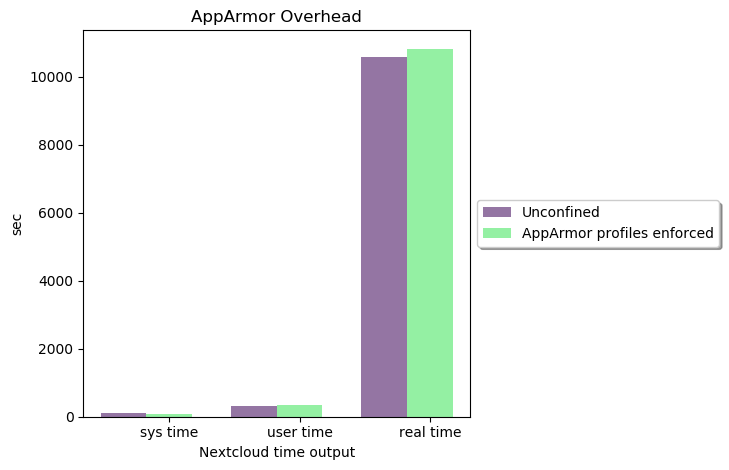
\includegraphics[width=1\linewidth]{figures/overhead.png}
%   \caption{AppArmor overhead}
\end{figure}

\hfill\break
\textbf{Απόδοση}
\hfill\break

Για να εξετάσουμε την απόδοση του \en SecureWilly\gr{} καταλήξαμε ότι δεν είχε νόημα να μετρήσουμε το χρόνο εκτέλεσης, γιατί εξαρτάται καθαρά από τον χρόνο εκτέλεσης του πλάνου χρήσης του \en docker project\gr{} που δέχεται ως είσοδο. Συνεπώς, αυτό που είχε νόημα να ελέγξουμε ήταν ο αριθμός των εκτελέσεων του πλάνου χρήσης εντός της δυναμικής ανάλυσης που χρειάστηκε για να λάβουμε τα τελικά \en profiles\gr{}. Έτσι για κάθε ένα από τα \en docker projects\gr{} δημιουργήσαμε διαγράμματα που αναπαριστούν την αύξηση των κανόνων του \en profile\gr{} του κάθε \en service\gr{} ανα \en run\gr{}.

Αυτό που παρατηρήσαμε στα διαγράμματα κανόνων ανα \en run\gr{} ήταν ένα κατώφλι (\en threshold\gr{}), πριν το οποίο τα \en services\gr{} συνεχώς αποκτούν νέους κανόνες ανα \en run\gr{}, ενώ κατά το κατώφλι αρχίζουν να σταθεροποιούνται και μόλις το περάσουν ακολουθούν δύο \en complain runs\gr{} που οδηγούν στο \en enforce run\gr{} που επιβεβαιώνει ότι δεν υπάρχουν νέοι κανόνες να εξαχθούν από τα \en logs\gr{} του συστήματος.

Στην παρακάτω εικόνα φαίνεται το διάγραμμα κανόνων \en profile\gr{} ανα \en run\gr{} για το \en media streaming benchmark\gr{}:

%\begin{center}{\en Media streaming\gr{}}\end{center}
\begin{figure}[H]
  \centering
   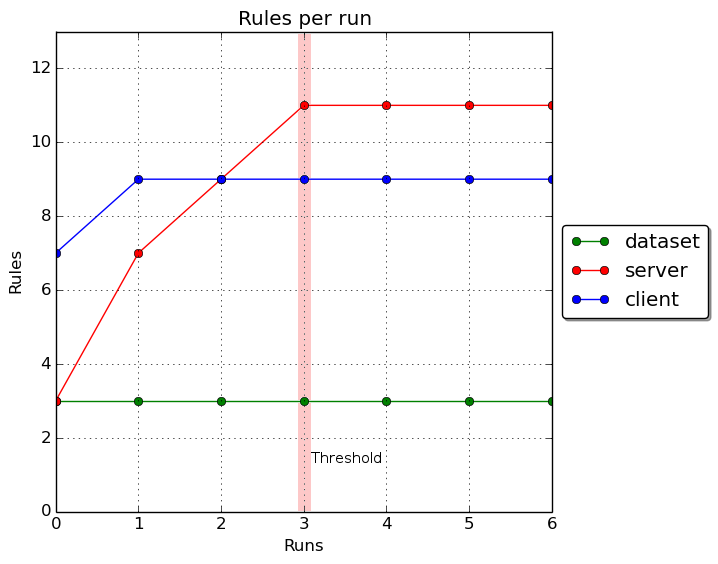
\includegraphics[width=0.75\linewidth]{figures/mediastreaming/rulesthreshold.png}
 %%%  \caption{Media Streaming: Rules per run for each service}
\end{figure}

Όπως φαίνεται και στο παρακάτω διάγραμμα όπου εμφανίζονται όλα τα \en docker projects\gr{} που δοκιμάσαμε, η θέση τόσο του \en threshold\gr{} όσο και του τελικού \en run\gr{} εξαρτάται από την πολυπλοκότητα του \en docker project\gr{}. Όσο περισσότερες λειτουργίες έχουν τα \en services\gr{}, τόσο περισσότεροι κανόνες απαιτούνται και τόσο περισσότερα \en runs\gr{} θα μεσολαβήσουν μέχρι το \en threshold\gr{} αλλά και μέχρι τα τελικά \en profiles\gr{}. 
\begin{figure}[H]
  \centering
   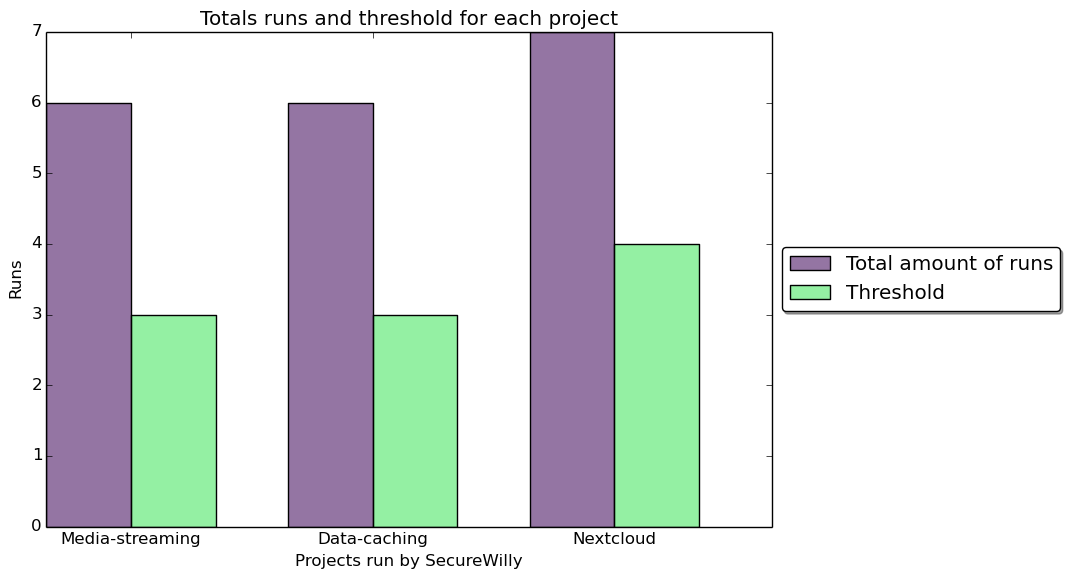
\includegraphics[width=0.85\linewidth]{figures/compare.png}
%%%   \caption{Comparing total runs and threshold between projects run by SecureWilly}
\end{figure}

\hfill\break
\textbf{Λειτουργικότητα}
\hfill\break

Η εξέταση της λειτουργικότητας του \en SecureWilly\gr{} στην πραγματικότητα ταυτίζεται με την εξέταση του πλάνου χρήσης, έχοντας τα \en profiles\gr{} που δημιουργήσαμε ενεργοποιημένα σε \en enforce mode\gr{} και ελέγχοντας αν επιτρέπονται όλες οι ενέργειες που περιλαμβάνονται σε αυτό.

Τα \en profiles\gr{} που παράγει άλλωστε το λογισμικό μας βασίζονται εξ'ολοκλήρο στις εντολές που περιλαμβάνει το πλάνο χρήσης, αφού δεν υπάρχει άλλος τρόπος να προβλέψουμε τις επιθυμητές ενέργειες που πρέπει να επιτρέπονται.

Το \en SecureWilly\gr{} κάνει ένα \en testing\gr{} στην λειτουργικότητα, μέσα στη δυναμική ανάλυση, αφού στο τέλος θέτει τα \en profiles\gr{} σε \en enforce mode\gr{} και επιβεβαιώνει ότι δεν παράγονται νέα \en logs\gr{} που οδηγούν σε καινούριους κανόνες.

Παρακάτω βλέπουμε για το \en data caching benchmark\gr{} το διάγραμμα κανόνων ανα \en run\gr{} επισημαίνοντας με διαφορετικό χρώμα τα \en runs\gr{} με \en complain\gr{} και με \en enforce mode\gr{}.

\begin{center}{\en Data caching\gr{}}\end{center}
\begin{figure}[h!]
  \centering
   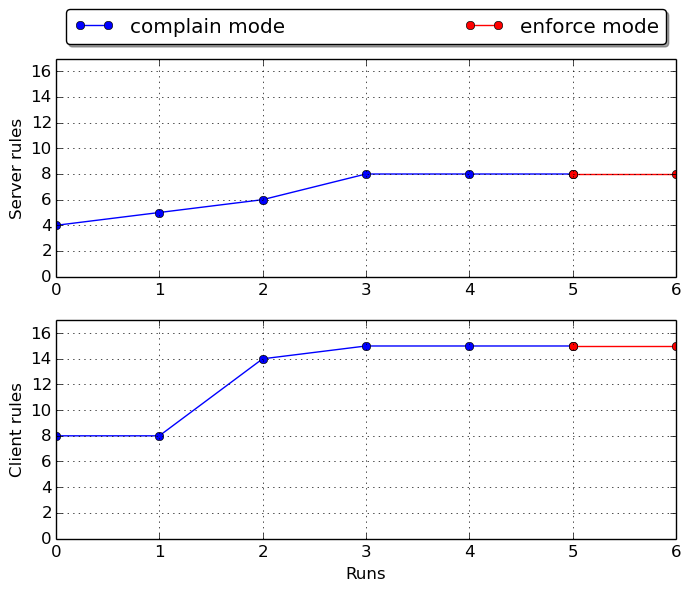
\includegraphics[width=0.75\linewidth]{figures/datacaching/complain_enforce_rules.png}
 %  \caption{Data Caching: Rules per run, emphasizing complain/enforce mode}
\end{figure}

Σε όλα από τα \en docker projects\gr{} που δοκιμάστηκαν, μόνο ένα \en run\gr{} σε \en enforce mode\gr{} χρειάστηκε, δηλαδή το πλάνο χρήσης δεν έδωσε \en logs\gr{} με νέους κανόνες προς εξαγωγή.

Ένας άλλος τρόπος για να αξιολογήσουμε τη λειτουργικότητα του \en SecureWilly\gr{} είναι μέσω των κανόνων του κάθε \en profile\gr{} που παράγει. Συγκεκριμένα, εξετάζουμε αν οι κανόνες αντικατοπτρίζουν τον ρόλο που έχει κάθε \en service\gr{} μέσα στο \en docker project\gr{}.

Για παράδειγμα, στα παρακάτω διαγράμματα βλέπουμε το \en Nextcloud instance\gr{} και τις διαφορετικές κατηγορίες κανόνων που εξάγονται για κάθε \en service\gr{}.

\begin{center}{\en Nextcloud server\gr{}}\end{center}
\begin{figure}[h!]
  \centering
   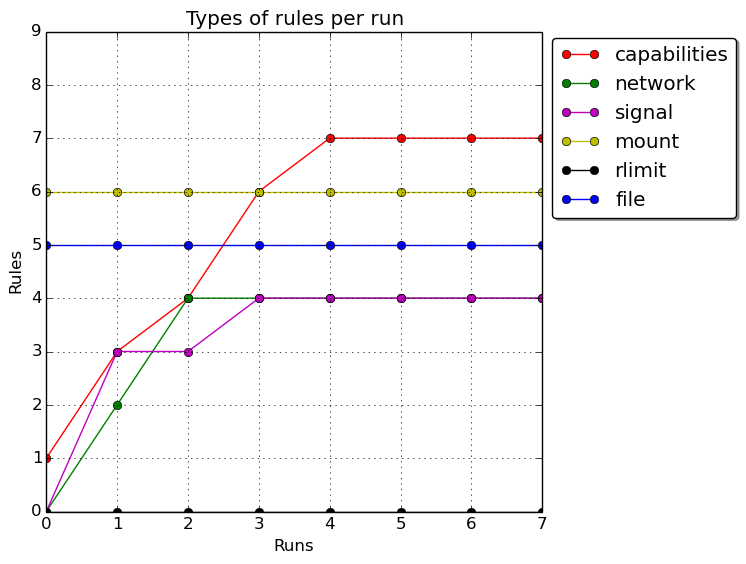
\includegraphics[width=0.68\linewidth]{figures/nextcloud/types_nextcloud.png}
  % \caption{Nextcloud: Nextcloud types}
\end{figure}

\begin{center}{\en Database service\gr{}}\end{center}
\begin{figure}[H]
  \centering
   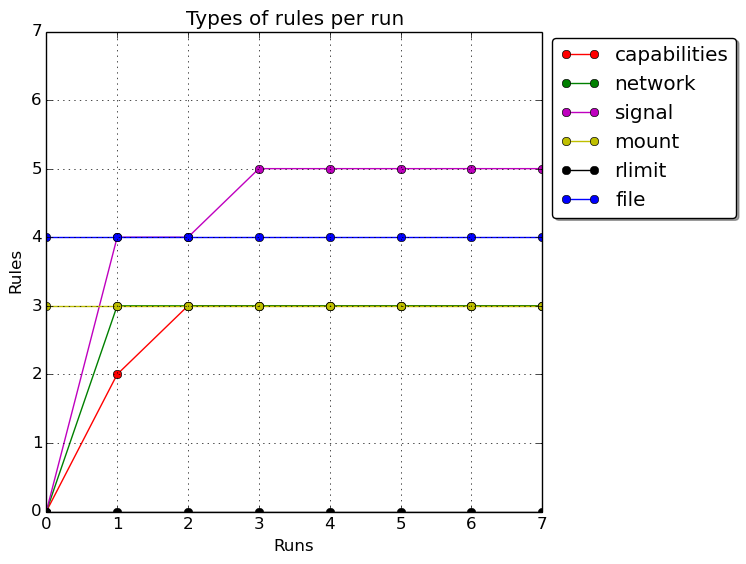
\includegraphics[width=0.68\linewidth]{figures/nextcloud/types_db.png}
 %  \caption{Nextcloud: Db types}
\end{figure}

Ο \en server\gr{} έχει πολλούς κανόνες τύπου \en capability\gr{} οι οποίοι αυξάνονται σταδιακά ανα \en run\gr{} και αυτοί καθορίζουν και τη θέση του \en threshold\gr{}, το οποίο οφείλεται στο γεγονός ότι ο \en server\gr{} είναι υπεύθυνος για να συνδεθεί με τη βάση δεδομένων και να υπηρετήσει όλους τους χρήστες. Οι κανόνες τύπου \en file\gr{} και \en mount\gr{} προστίθενται στην στατική ανάλυση, λόγω των \en volumes\gr{} και παραμένουν σταθεροί για όλα τα υπόλοιπα \en runs\gr{}. Επιπλέον, χρειάζονται κάποιοι κανόνες τύπου \en network\gr{}, όπως σχεδόν σε όλα τα \en multi-service projects\gr{}, ώστε να μπορούν να επικοινωνούν τα \en services\gr{} μεταξύ τους - στο παράδειγμα μας ο \en server\gr{} με τη βάση δεδομένων - καθώς και κάποιοι κανόνες τύπου \en signal\gr{} ώστε να μπορούμε να τερματίσουμε τα \en containers\gr{}.

Το \en service\gr{} της βάσης δεδομένων χρειάζεται επίσης κάποιους κανόνες τύπου \en capability\gr{}, αλλά λιγότερους από ότι ο \en server\gr{}. Χρειάζεται επίσης μερικούς κανόνες τύπου \en signal\gr{} για να μπορεί να χειριστεί τα σήματα τερματισμού καθώς και κανόνες \en network\gr{} που καθιστούν εφικτή την επικοινωνία με τον \en server\gr{}. Ωστόσο, το \en profile\gr{} της βάσης δεδομένων απαρτίζεται κυρίως από κανόνες \en file\gr{} και \en mount\gr{}, λόγω των \en volumes\gr{} που χειρίζεται και την πρόσβαση σε αρχεία που χρειάζεται, κάτι το οποίο είναι και θεμελιώδες χαρακτηριστικό μιας βάσης δεδομένων.

\hfill\break
\textbf{Επεκτασιμότητα}
\hfill\break

Η επεκτασίμοτητα του \en SecureWilly\gr{} δοκιμάστηκε στο \en benchmark media streaming\gr{} αυξάνοντας τον αριθμό των \en client services\gr{}. Σε αυτό το σημείο παρατηρήσαμε ότι το \en SecureWilly\gr{} μπορεί να χειριστεί μεγάλες επεκτάσεις ενός \en project\gr{} που αφορούν τον αριθμό των \en services\gr{} και η παραγωγή των \en profiles\gr{} δεν επηρεάζεται με κανέναν τρόπο από αυτήν. Ο χρόνος φυσικά όπως είναι αναμενόμενο θα αυξηθεί ανάλογα με την χρονική αύξηση του πλάνου χρήσης.

Μια μελλοντική επέκταση του \en SecureWilly\gr{} θα μπορούσε να περιλαμβάνει και τη διαχείριση ενός κατανεμημένου συστήματος, όπου το \en docker project\gr{} θα περιλαμβάνει \en containers\gr{} που τρέχουν σε διαφορετικά μηχανήματα. Σε αυτήν την περίπτωση, το \en SecureWilly\gr{} θα τρέχει σε ένα από αυτά τα μηχανήματα και θα ζητάει από τα υπόλοιπα να του στείλουν τα \en logs\gr{} που παράχθηκαν για το εκάστοτε \en profile\gr{} που έτρεξε, ενώ στο τέλος θα τους παρέχει το τελικό \en profile\gr{} που δημιουργήθηκε. Η διαδικασία αυτή φαίνεται στο παρακάτω σχήμα:
\begin{figure}[H]
  \centering
   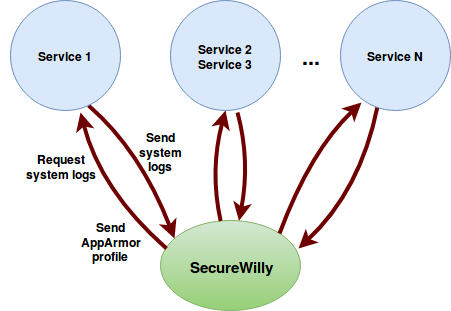
\includegraphics[width=0.6\linewidth]{figures/DistributedSystems.png}
  % \caption{SecureWilly handling distributed services}
\end{figure}

\section*{Επίλογος}

Η διατήρηση της ασφάλειας και συγκεκριμένα της απομόνωσης στα \en docker containers\gr{}, όπως και η αποφυγή επιθέσεων είναι πολύ απαιτητικές διαδικασίες. Μάλιστα η διαδικασίες αυτές γίνονται ακόμα πιο περίπλοκες όταν προσπαθούμε να εξισορροπήσουμε την ασφάλεια ενός \en docker container\gr{} με την λειτουργικότητα του.

Στην παρούσα διπλωματική ασχοληθήκαμε με την ασφάλεια σε περιβάλλον \en docker\gr{} από μια πρακτική οπτική, καθώς δημιουργήσαμε ένα λογισμικό που παράγει με αυτόματο τρόπο \en AppArmor profiles\gr{} για ένα \en docker project\gr{}. Τα \en profiles\gr{} αυτά είναι προσαρμοσμένα στο δοσμένο \en docker project\gr{} και αποτελούνται από τους λιγότερους δυνατόν κανόνες που καθιστούν ένα \en profile\gr{} ασφαλές και αποδοτικό, με βάση την Αρχή των Ελάχιστων Προνομίων. Αυτό σημαίνει ότι επιτρέπεται αποκλειστικά μια ομάδα ενεργειών ενώ κάθε άλλη ενέργεια θα μπλοκάρεται, αφού θα θεωρείται περιττή. Η ομάδα ενεργειών που επιτρέπεται καθορίζεται από το χρήστη, μέσω του πλάνου χρήσης που παρέχει σαν είσοδο. Το λογισμικό μας μπορεί να διαχειριστεί τόσο \en single\gr{} όσο και \en multi service docker projects\gr{} και τα \en profiles\gr{} που δημιουργούνται είναι προσανατολισμένα στο κάθε \en service\gr{}. Επομένως, κάθε \en service\gr{} έχει το δικό του \en profile\gr{}, πράγμα που κάνει το \en profile\gr{} πολύ συγκεκριμένο σχετικά με τη λειτουργία του \en service\gr{} αλλά με γνώση της συνεργασίες του με τα υπόλοιπα \en services\gr{}. 

Εκτός από το λογισμικό που δημιουργήσαμε, στην παρούσα διπλωματική, παρουσιάζουμε μια εκτενή έρευνα πάνω στα ευπαθή χαρακτηριστικά του \en docker\gr{} που θα μπορούσαν να οδηγήσουν στην παραβίαση της απομόνωσης των \en containers\gr{} και υλοποιούμε μια σειρά από παραδείγματα για επιθέσεις τύπου \en container breakout\gr{}, στα πλαίσια του ηθικού \en hacking\gr{}, που δημιουργήσαμε προκειμένου να βοηθήσουμε στην πρόληψη επιθέσεων αυτού του τύπου, μέσω του λογισμικού μας.

Τέλος, προκειμένου να αξιολογήσουμε το λογισμικό μας ως προς τη λειτουργικότητα, την απόδοση και την επεκτασιμότητα χρησιμοποιήσαμε κάποια \en benchmarks\gr{} του \en Cloudsuite\gr{} και ένα \en instance\gr{} του \en Nextcloud\gr{}. Καταφέραμε με επιτυχία να δημιουργήσουμε \en AppArmor profiles\gr{} για τα \en services\gr{} αυτών, ελπίζοντας πως συνεισφέραμε με αυτόν τον τρόπο στις αντίστοιχες κοινότητες. Επίσης συγκρίναμε τα \en profiles\gr{} που δημιουργήσαμε με αυτά του \en genprof\gr{} εργαλείου και εντοπίσαμε τις διαφορές μεταξύ τους. Η χρονική καθυστέρηση εξαιτίας του \en AppArmor\gr{} γενικότερα αποδείχθηκε ότι είναι τόσο μικρή που μετα βίας μπορεί να γίνει αντιληπτή και έτσι καταλήξαμε στο συμπέρασμα ότι το \en SecureWilly\gr{} παράγει αξιόλογα εργαλεία προκειμένου να ενισχύσει την ασφάλεια ενός \en docker project\gr{}.
\en
